%\subsection{Neocortical Layer 4/5 Pyramidal Cell Test Suite}
\subsubsection{Performance of Layer 5 Prefrontal cortex Pyramidal Neuron on NeuronUnit tests of model data agreement}

A suite of neuronunit tests containing the tests: rheobase value, membrane voltage time constant ($tau_{m})$, input resistance was computed. This multi-compartment, conductance based model served as a useful benchmark, for us to evaluate the relative performance of reduced model fits.
    
\begin{figure}    
\begin{center}
    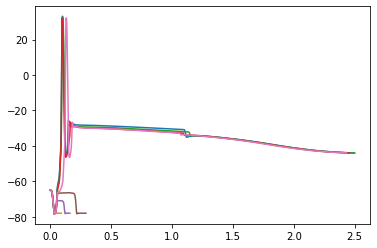
\includegraphics[width=0.7\linewidth]{figures/NU_BBP_fusion_L5PC_files/NU_BBP_fusion_L5PC_3_1.png}
\end{center}
\end{figure}  

It is worth noting that the layer 5 neocortical pyramidal neuron was very slow to dispatch relative to the reduced models developed in this thesis work. Where as a typical reduced model described here evaluated in the order of $~0.0025 seconds$, this model on average took $5.74$, for a single run and $34.8$ to solve for the models Rheobase, current.

\begin{table}[ht]
\centering
\resizebox{\textwidth}{!}{
\begin{tabular}{lllllll}
\toprule
{} & RheobaseTest & InputResistanceTest & TimeConstantTest & CapacitanceTest & InjectedCurrentAPWidthTest & InjectedCurrentAPThresholdTest \\
\midrule
0 &     Z = 0.07 &           Z = -0.90 &         Z = 0.14 &        Z = 1.29 &                  Z = -1.98 &                      Z = -2.09 \\
\bottomrule
\end{tabular}}
\end{table}

In this pre-optimized model, only the rheobase test, and the time constant test seemed to fall within the range of biological plausibility.